
%(BEGIN_QUESTION)
% Copyright 2006, Tony R. Kuphaldt, released under the Creative Commons Attribution License (v 1.0)
% This means you may do almost anything with this work of mine, so long as you give me proper credit

Define the following terms as they apply to the level controller shown in this P\&ID (LIC 135), controlling the level of liquid in the horizontal receiver vessel:

$$\includegraphics[width=15.5cm]{i00135x01.eps}$$

\begin{itemize}
\item{} Process Variable (PV)
\item{} Setpoint (SP)
\item{} Manipulated Variable (MV)
\item{} Process alarm
\end{itemize}

\underbar{file i00135}
%(END_QUESTION)





%(BEGIN_ANSWER)

\begin{itemize}
\item{} Process Variable (PV) = The signal representing liquid level in the horizontal vessel
\item{} Setpoint (SP) = The point at which the controller tries to maintain the liquid level inside the vessel
\item{} Manipulated Variable (MV) = The controller's output signal, which tells the control valve how far to open or close, thus influencing the amount of liquid exiting the vessel at the bottom.
\item{} Process alarm = level indicator (LI) does double-duty as a high- and low-alarm unit in addition to being an indicator for the operators.  We know this from the ``LAL'' and ``LAH'' labels near the bubble.
\end{itemize}

\vskip 10pt

Incidentally, the ``LG'' instrument on the left-hand side of the receiver vessel is a {\it level gauge}, also known as a {\it sightglass}.  It is used for manual inspection of vessel level.

%(END_ANSWER)





%(BEGIN_NOTES)

\vskip 20pt \vbox{\hrule \hbox{\strut \vrule{} {\bf Virtual Troubleshooting} \vrule} \hrule}

This question is a good candidate for a ``Virtual Troubleshooting'' exercise.  Presenting the diagram to students, you first imagine in your own mind a particular fault in the system.  Then, you present one or more symptoms of that fault (something noticeable by an operator or other user of the system).  Students then propose various diagnostic tests to perform on this system to identify the nature and location of the fault, as though they were technicians trying to troubleshoot the problem.  Your job is to tell them what the result(s) would be for each of the proposed diagnostic tests, documenting those results where all the students can see.

During and after the exercise, it is good to ask students follow-up questions such as:

\begin{itemize}
\item{} What does the result of the last diagnostic test tell you about the fault?
\item{} Suppose the results of the last diagnostic test were different.  What then would that result tell you about the fault?
\item{} Is the last diagnostic test the best one we could do?
\item{} What would be the ideal order of tests, to diagnose the problem in as few steps as possible?
\end{itemize}


%INDEX% Basics, signal label: manipulated variable (MV) 
%INDEX% Basics, signal label: process variable (PV) 
%INDEX% Basics, signal label: setpoint (SP) 
%INDEX% Process: receiver vessel liquid level control (generic)

%(END_NOTES)


